\clearpage

\section{Oxford Nanopore: cDNA Sequencing}
%https://www.nature.com/articles/s41587-020-0731-9

\subsection{Introduction}
In 2014, Oxford Nanopore Technology (ONT) introduced another long-read sequencing technology akin to PacBio's SMRT with the ability to also generate long reads capable of resolving the exon structure of mRNA transcripts. However, rather than mimicking the natural DNA synthesis and measuring the incorporation events on the template strand (as is the focus in all major sequencing applications including the PacBio's SMRT) ONT's nanopore-based sequencing adopted an entirely novel approach by directly inferring the DNA sequence in real-time from electric current fluctuations as the DNA translocates through a protein pore. 

\subsubsection{Mechanism}
In contrast to Pacbio's XXX by XXX Sequel, ONT's nanopore sequencing can be performed in a handheld MinION device (10 × 3 × 2 cm, 90 g), housing a flow cell at its centre where the DNA sample is loaded. (Also on mobile device: \cite{Samarakoon2020}) Each flow cell contains a sensor array, consisting of 512 channels, each with 4 cells that can in turn house one nanopore (currently CsgG pore from \textit{E.coli} \cite{Goyal2014}), which is inserted in an electrical resistant membrane surrounded by electrolytes. As an electric field is applied across the membrane, the negatively-charged DNA is driven across the nanpopore and subsequently interrupts the current. Different nucleotides would disrupt the electrical currenly differently, thereby generating a signal that is nucleotide-sensitive and a proxy of the DNA sequence. However, while the current MinION contains a total of 2048 nanopores, only one of the four wells in each channel can be active at any time, as controlled by Application Specific Integrated Circuit (ASIC), allowing up to 512 independent DNA molecules to be sequenced simultaneously.

*6-mer* 
*flow cell and the different nanopore?*
% https://genomebiology.biomedcentral.com/articles/10.1186/s13059-018-1462-9
% https://community.nanoporetech.com/posts/flo-minxxx-x-rx-x-r
%The difference is in the nanopores present in each flow cell. The nanopore is essentially a biological protein; it is found naturally occurring in the environment. We perform a lot of engineering internally to optimise these nanopores for utilisation in our system, enabling greater throughput and accuracy. The R9.4.1 nanopore is the current broadly-used nanopore. As DNA moves through the nanopore, there's a pinch-point - a narrowing of the hole, which allows us to measure the current, and so interpret the translocation of the molecule in real time. In the R10 series, there is a longer barrel and two pinch points, enabling two such measurements. This provides benefits for the sequencing of homopolymers - stretches of the same base multiple times. These homopolymer stretches are difficult, not only for our platform, but for all sequencing plaforms. We have found that introducing this second pinch point provides better fidelity for homopolymer sequences than previously seen with the R9.4 series; we are starting to see very accurate sequencing of homopolymer stretches of about ten bases. R10.3 is the newest nanopore in this series, and provides the high accuracy of the R10 series together with increased throughput and capture.
%https://nanoporetech.com/sites/default/files/s3/Product_brochure_Final_July_2018.pdf
%https://community.nanoporetech.com/posts/flowcell-r9-5-and-1dsq-lib
%https://community.nanoporetech.com/posts/1d-2-cdna-library-prep-low
%https://link.springer.com/content/pdf/10.1007%2F978-1-4939-7834-2.pdf

\subsubsection{Performance and Run Quality Metric}
The ability of nanopore sequencing to directly read the DNA has both positive and negative implications. Inhibited mostly by the ability to deliver very high-molecular weight DNA to the pore, nanopore sequencing is able to generate much longer reads than SMRT sequencing (from 500bp to currently XXX), with theoretically no upper limit \cite{Loman2015}, and with no bias towards length or GC content \cite{Oikonomopoulos2016, Weirather2017}. This offers great potential in transcriptomics profiling and genome assembly. However without the circular feature of PacBio SMRT sequencing, DNA strand cannot be sequenced multiple times and one of the major limitations of nanopore sequencing is its lower read accuracy. Low complexity stretches, including homopolymers, are furthermore difficult to resolve as translocation of homopolymers do not change the sequence of nucleotides within pore, thereby resulting in a constant signal. 

%In contrast to PacBio's SMRT with the ability to generate consensus long reads, the raw accuracy of nanopore 1D cDNA sequencing is relatively low between 85–87\%; however, significant improvements are made on reducing error rate by rapid development of both the technology and library preparation methods (Volden et al. 2018). Such high error rates, from frequent base deletions and insertions particularly near splice sites, can result in spurious alignments and in correct clustering of reads. 

However over recent years, major advances in both the basecalling algorithms, the chemistry and nanopore itself has drastically increased the initial accuracy from 60\% \cite{Jain2015} to 98.3\% (vR.9.4.1 and Bonito). This includes the chemistry (1D\textsuperscript{2}) to sequence both the template and the complementary strand immediately after, thereby attaining a more accurate consensus read that increases the accuracy of template reads (1D) alone by 5\%\cite{Rang2018}. Further to mimic the circular consensus approach, two methodologies (INC-seq \cite{Li2016c} and R2C2 \cite{Volden2018}) involving Rolling Circle Amplification and subsequent nanopore sequencing of circularised templates have been proposed with accuracy approaching 97.5\%. 

\subsection{Lab Pipeline}
\label{chap:ont_labpipeline}
Similar to the Iso-Seq library preparation (Chapter \ref{chap:isoseq_labpipeline}), nanopore sequencing of transcriptome also involved three main steps by first generating and amplifying cDNA, finally followed by ligation of adaptors. However unlike PacBio whereby the polymerase is bound after ligation of adaptors, the molecular motor (that drives the DNA through the pore) is already bound to the adaptors. At the time I trialled the nanopore sequencing, the Iso-Seq Express Library Preparation protocol had not yet been released, and the ONT rapid library preparation was much shorter and simpler than the Iso-Seq protocol I used.    

\begingroup
\parindent=0em
\etocsettocstyle{\rule{\linewidth}{\tocrulewidth}\vskip0.5\baselineskip}{\rule{\linewidth}{\tocrulewidth}}
\etocsetnexttocdepth{5}
\localtableofcontents 
\endgroup

\subsubsection{cDNA synthesis}
For a fair, direct comparison between ONT's MinION sequencing and PacBio's IsoSeq, 200ng total RNA extracted using AllPrep DNA/RNA Mini Kit (Qiagen) was likewise converted to single-stranded DNA using SMARTer PCR cDNA Synthesis(ClonTech).

\subsubsection{ONT MinION Library Preparation}
Despite a range of protocols available on the Oxford Nanopore community protocol that can be used pending on the source of sample, the SQK-LSK109 kit was used with cDNA as starting material. This kit is PCR-free and as such is dependent upon generation of high-quality and full-length cDNA, which would be provided using the SMARTer PCR cDNA synthesis kit rather than that detailed in 1D Strand switching cDNA by ligation protocol (SQK-LSK108).

\subsubsection{Repair DNA and Ends}
DNA calibration strand (DCS) is 3.6kb amplicon of Lambda genome, and is included in the sample library as a quality control of base-calling and sample preparation. End Repair prepare the ends of cDNA molecules for adapter attachment by addition of dA nucleotides

\subsubsection{Adapter Ligation}
Post DNA repair and end repair, ONT adapters with dT overhang are ligated to the 5’ end of the dA-tailed cDNA molecules by hybridisation. The ONT adapters contain: 
\begin{itemize}
	\item motor protein (loaded processive enzyme?) that can bind to the nanopore and control/increase the speed of DNA translocation through the pore. While it is active in solution, it is inhibited from contacting the rest of the DNA through specialised bases in the adapter.
	\item cholesterol tether to facilitate DNA capture as (1) tethers the DNA molecule to the lipid bilayer (membrane) of the flow cell  (2) reduces amount of diffusion of the DNA molecule from three dimensions (i.e the volume of whole buffer) to two dimensions (i.e. across the lipid bilayer)  
\end{itemize}

\subsubsection{Priming the Flow Cell}
Sequencing buffer provides the optimal chemical conditions for powering DNA translocation through the Nanopore. This is the substrate cofactor of the motor enzyme that is used for DNA translocation process in the pore. 

\newpage
\subsection{Bioinformatics Pipeline}
This section describes the bioinformatic pipeline that was used to process ONT cDNA sequencing data generated using the whole transcriptome (n = 2) in \cref{ch: whole_transcriptome} and targeted transcriptome approach (n = 20) \cref{ch: targeted_transcriptome}. 

Unlike the Iso-Seq bioinformatics pipeline which was largely established by PacBio (described in \cref{section:isoseq_bioinformatics}, \cref{fig:isoseq_bioinformatics_Pipeline}), the bioinformatics pipeline for processing ONT raw reads was less defined and streamlined. While significant improvements in bioinformatic tools have been released by ONT over the last 2 years, many of the new tools were only applicable to sequencing data generated from ONT-specific protocols and primers. Consequently, given that ONT sequencing data in this thesis was generated using the same primers and barcodes as Iso-Seq sequencing data for a fairer comparison, the initial stage of the bioinformatics pipeline was adapted from the Wellcome Trust Advanced Course: RNA Transcriptomics (2018), provided by J.Ragoussis (referred as WTAC), and refined using ERCC as benchmark. Many of the downstream tools developed for Iso-Seq were then similarly applied for the latter stage of ONT bioinformatics pipeline, bar the substitution of \textit{TAMA} for \textit{Cupcake} for transcript collapse (\cref{fig:ONT_PacBio_bioinformatics}). 

The steps for processing sequencing data from the whole and targeted transcriptome approach is largely similar, with the exception of an additional step of barcode demultiplexing in the targeted approach as 10 samples were barcoded and sequenced simultaneously in one flow cell (\cref{fig:ONT_Targeted_bioinformatics}). 

\begingroup
\parindent=0em
\etocsettocstyle{\rule{\linewidth}{\tocrulewidth}\vskip0.5\baselineskip}{\rule{\linewidth}{\tocrulewidth}}
\etocsetnexttocdepth{5}
\localtableofcontents 
\endgroup

\begin{figure}[htp]
	\centering
	\includegraphics[page=15,trim={0cm 6cm 0cm 0cm},clip,scale = 0.8]{Figures/ProjectDevelopment_Figures}
	\captionsetup{width=0.95\textwidth,singlelinecheck=off}
	\caption[Comparison of bioinformatics pipeline for processing PacBio Iso-Seq and ONT 1D-reads]%
	{\textbf{Comparison of bioinformatics pipeline for processing PacBio Iso-Seq and ONT 1D-reads}. Shown is a side-by-side comparison of the bioinformatics pipeline used to process PacBio Iso-Seq and ONT 1D-reads from initial processing of raw reads, alignment to reference genome with \textit{Minimap2}, collapse of reads to transcripts followed by annotation with \textit{SQANTI}. The bioinformatic pipelines adopted are largely similar between Iso-Seq and ONT with the difference primarily in the initial processing of raw reads; raw Iso-Seq reads were processed with \textit{Iso-Seq3} tool (PacBio) whereas raw ONT reads were processed with various community-based packages.   
	}
	\label{fig:ONT_PacBio_bioinformatics}
\end{figure}

\begin{figure}[htp]
	\centering
	\includegraphics[page=16,trim={0cm 6cm 0cm 0cm},clip,scale = 0.8]{Figures/ProjectDevelopment_Figures}
	\captionsetup{width=0.95\textwidth,singlelinecheck=off}
	\caption[Bioinformatics Pipeline for ONT Targeted Transcriptome]%
	{\textbf{Bioinformatics Pipeline for ONT Targeted Transcriptome}. Shown is a detailed bioinformatics pipeline for processing ONT reads 1D reads from the targeted transcriptome, whereby 20 samples were barcoded and sequenced simultaneously on two flow cells (referred as Batch 2 and Batch 3 of the original Iso-Seq Targeted Transcriptome set). Supplementing \cref{fig:ONT_PacBio_bioinformatics}, raw ONT reads from each flow cell were processed and the demultiplexed into the respective samples, which were then processed independently for collapse and transcript quantification. All the samples from both batches were then merged into one complete dataset, while retaining sample-specific transcript expression. 
	}
	\label{fig:ONT_Targeted_bioinformatics}
\end{figure}


\subsubsection{Quality Control of Run, Base-calling and Filtering of Base-called Reads}
The performance of a Nanopore sequencing run was assessed using \textit{PycoQC}\cite{Leger2019} and the official Nanopore QC tutorial\cite{ONT2019NanoporeQC}, by evaluating the number of active pores during the run, the number of reads generated over time, and the length and quality score distribution of basecalled reads. A suboptimal run would be indicated by a low sequencing yield (<20kb), whereby the vast majority of pores were inactive or there was significant increase in the number of inactive pores over time. 

Raw reads were basecalled using \textit{Guppy}, a basecaller program which converts ONT's raw electrical signal to DNA sequence. Basecalling is a rapidly advancing field current basecallers developed by using neural networks and training machine-learning algorithms on real data\cite{Wick2019}. The latest released basecaller by ONT, Guppy has been shown to perform superior to other available basecallers with higher read accuracy and faster basecalling\cite{Wick2019}. Basecalled reads with read quality score < 7 were then removed using \textit{Nanofilt}\cite{DeCoster2018} with default parameters. 


\subsubsection{Removing of Nanopore and cDNA sequencing adapters}
Similarly to the Iso-Seq bioinformatics pipeline, cDNA sequencing primer sequences and nanopore ligation adaptors were removed to prevent spurious alignment, using \textit{Porechop}\cite{Wick2017} (v0.2.4, parameters: --end\_size 100, --adapter\_threshold 90, --end\_threshold 75, --min\_trim\_size 15, --discard\_middle, --extra\_end\_trim 1). Under those parameters, a window of 100 nucleotides from each end of the reads were searched for a set of adaptors, which must have a minimum 90\% identity to be considered present for trimming and a minimum 75\% at the end of the reads; alignments smaller than 15bp or found within the middle of the reads (considered chimeric) were removed. By manually defining a unique set of adaptors that includes the cDNA primers (from Clontech SMARTer PCR cDNA synthesis kit), the ONT adaptors and corresponding polyA/T tail, it was possible to differentiate the strand orientation (\cref{fig:ONT_cdnatemplate}); the adapter sequences used for whole transcriptome and targeted transcriptome approach are given in \cref{fig:ONT_cdnatemplate}\textbf{b} and \cref{tab:ont_barcode} respectively. Sample demultiplexing in the targeted transcriptome approach was performed by including the 16bp barcode sequence; of note, the barcode is only present in the 3'end of the plus strand and 5'end of the minus strand, as part of the oligo-dT primer during cDNA synthesis (\cref{tab:barcode_primers}). Reads were therefore assigned to the sample with the highest identity at the 5'end and 3'end for the plus and minus strand respectively. 

\textit{Porechop} has been officially unsupported since 2018 and has been largely replaced by ONT's officially recommended tool, \textit{Pychopper}\cite{OxfordNanoporePychopper}. While \textit{Pychopper} is useful for ONT-specific barcode demultiplexing, it was not able to differentiate and orient reads from the plus and minus strand without unique sequences. Given that the ONT cDNA reads were generated using the SMARTer cDNA synthesis kit (Clontech) (described in \cref{section:ch2_cDNA_synthesis_explanation}), 5’ end of the plus and minus strands are reverse complements of each other with the only difference being that the plus strand ends with ATGGG and the minus strand ends with polyT (\cref{fig:ONT_cdnatemplate}). 

Trimmed reads with adaptors present at both ends were retained, and reads corresponding to the minus strand were reverse complemented. Using \textit{Cutadapt}\cite{Martin2011} (v2.9, -a "A{40}"), the polyA sequence was then trimmed 40 nucleotides from the 3'end.



\begin{figure}[ht]
	\begin{center}
		\includegraphics[page=7,trim={0cm 17cm 0cm 1cm},clip, scale = 0.7]{Figures/ProjectDevelopment_Figures.pdf}
	\end{center}
	\captionsetup{width=0.95\textwidth}
	\caption[Structure of ONT library cDNA template]%
	{\textbf{Structure of ONT library cDNA template}: Shown is the \textbf{a)} final structure of cDNA molecules for ONT sequencing, after cDNA synthesis and adaptor ligation, and the corresponding differentiating start and end sequence for the plus and minus strands \textbf{b)} without and \textbf{c)} with barcodes. The original cDNA molecules are outlined in purple and green, and the ONT boxes indicate the position of the ONT adaptors. In cases where multiplexing is performed, the barcode location is indicated in red (see \cref{tab:barcode_primers} and \cref{tab:ont_barcode} for barcode sequences). Of note, only the plus strand end sequence and the minus strand start sequence contain the barcode and are used for sample demultiplexing, whereas the plus strand start and minus strand end sequence are identical across all barcoded samples. The brown and orange circle refer to the motor protein and cholesterol moiety respectively. The start and end of the strand is defined by the 5' and 3' end respectively. }
	\label{fig:ONT_cdnatemplate}
\end{figure}

\begin{landscape}
	\begin{table}[]
		\centering
		\begin{tabular}{@{}ccccc@{}}
			\toprule
			\multirow{2}{*}{Barcoded  Samples} & \multicolumn{2}{c}{Plus strand} & \multicolumn{2}{c}{Minus strand} \\ \cmidrule(l){2-5} 
			& Start sequence & End sequence & Start sequence & End sequence \\ \midrule
			BC1 & \multirow{10}{*}{\begin{tabular}[c]{@{}c@{}}TTGCTAAG\\ CAGTGGTA\\ TCAACGCA\\ GAGTACAT\\ GGG\end{tabular}} & AAAAAACGCACTCTGATATGTGGCA & CACATATCAGAGTGCGTTTTTT & \multirow{10}{*}{\begin{tabular}[c]{@{}c@{}}CCCATGTAC\\ TCTGCGTTG\\ ATACCACT\\ GCTTAGCAAT\\ ACGTAACT\end{tabular}} \\
			BC2 &  & AAAAAAACTCACAGTCTGTGTGTGCA & ACACACAGACTGTGAGTTTTTTT &  \\
			BC3 &  & AAAAAAACTCTCACGAGATGTGTGCA & ACACATCTCGTGAGAGTTTTTTT &  \\
			BC4 &  & AAAAAAACGCGCGTGTGTGCGTGGCA & CACGCACACACGCGCGTTTTTTT &  \\
			BC5 &  & AAAAAAAACGCGAGAGTCGAGTGGCA & CACTCGACTCTCGCGTTTTTTTT &  \\
			BC6 &  & AAAAAAAACAGCTGATATATATGGCA & CATATATATCAGCTGTTTTTTTT &  \\
			BC7 &  & AAAAAAACACATAGAGATACAGAGCA & TCTGTATCTCTATGTGTTTTTTT &  \\
			BC8 &  & AAAAAAACGCAGCGCTCGACTGTGCA & ACAGTCGAGCGCTGCGTTTTTTT &  \\
			BC9 &  & AAAAAAATCTGTCTCGCGTGTGTGCA & ACACACGCGAGACAGATTTTTTT &  \\
			BC10 &  & AAAAAAACTCTGAGATAGCGCGTGCA & ACGCGCTATCTCAGAGTTTTTTT & 
		\end{tabular}
		\captionsetup{width=0.9\linewidth}
		\caption[ONT adapter sequences for plus and minus strand of barcoded samples]%
		{\textbf{ONT adapter sequences for plus and minus strand of barcoded samples}. Tabulated are the sequences used in \textit{Porechop} for sample demultiplexing and identifying the plus and minus strands. As depicted in \cref{fig:ONT_cdnatemplate}, only the plus strand end sequences and the minus strand start sequences contain the sample-specific barcode sequence (reverse complementary of one another). BC - Barcode}
		\label{tab:ont_barcode}
	\end{table}
\end{landscape}

\subsubsection{Genome Alignment and Transcript Collapse}
Trimmed reads were then aligned to the reference genome using Minimap2 \cite{Li2018} (v2.17-r941, parameters: -ax splice). In the Iso-Seq bioinformatics pipeline, mapped transcripts were then processed using \textit{Cupcake} for the removal of transcripts with low alignment identity and length, further collapse of high-quality transcripts to unique isoforms, and to obtain count information using output from \textit{Iso-Seq3 Cluster}.

As a similar comparison, mapped transcripts from ONT were processed using \textit{TAMA} for removal of lowly-aligned transcripts and for further collapse to unique isoforms (script: tama\_collapse.py, parameters: -e common\_ends, -c 95, -i 80, -x capped -a 50, -z 50, -m 20, -d merge\_dup) and to subsequently obtain count information (script: tama\_read\_support\_levels.py). Under those parameters recommended by WTAC, transcripts were filtered for minimum alignment identity > 80\% and alignment length >95\% (same threshold as that applied in Iso-Seq pipeline using \textit{Cupcake}) and collapsed by common exon start and end sites. 50 nucleotides at both 5'end and 3' end of the transcript, and 20 nucleotides at the exon/splice junction and tolerated for grouping transcripts to be collapsed. Of note, this is much more relaxed than the default \textit{TAMA} parameters (-a 10 -m 10 -z 10), given that the 5'cap method was not used and the error rate of ONT reads were high. 

Despite the growing emergence of various new tools developed for processing ONT reads - such as ONT's officially recommended pipeline with Pinfish and Stringtie, FLAIR, UNAGI - I chose to use \textit{TAMA} due to greater flexibility and transparency with parameter usage, generation of multiple output files for quality control, and ability to subsequently obtain count information (script: tama\_read\_support\_levels.py)


%\uline{\textbf{FLAIR}}: Full-Length Alternative Isoform analysis of RNA  (FLAIR\nomenclature{FLAIR}{Full-Length Alternative Isoform analysis of RNA}) 
%Three steps are involved: Correct splice sites with short reads if incorrect splice site is within 10base pairs away from correct splice site, collapse reads to generate consensus sequences. This involves first grouping reads with identical splice junctions - "first pass nanopore isoform transcriptome"; the representative isoform within each group is determined by the most supported transcription and end site. All the reads, including reads that were aligned but not able to be fully corrected, are re-aligned to the "first-pass isoform" with the best alignment. First-pass isoforms that have fewer than three supporting reads are filtered out; three supporting reads selected as threshold as this gave the highest base sensitivity without compromising on precision.  

\subsubsection{Transcriptome annotation \& Isoform abundance } 
In contrast to Iso-Seq, isoform quantification from ONT is relatively simpler in that each nanopore read corresponds to a single transcript (Tang et al. 2020). However, ambiguity still remains with assignment of truncated reads 

